\section{Introdução}\label{sec:intro}
\AtBeginSec

\begin{frame}{Elementos da Comunicação}
\begin{bigitem}
 \item A comunicação faz parte de nossa rotina diária:
 \begin{bigitem}
  \item chamada de telefone fixo ou móvel;
  \item e-mail na Internet;
  \item um programa de TV ou de rádio.
 \end{bigitem}
 \begin{figure}[!htb]
    \centering
    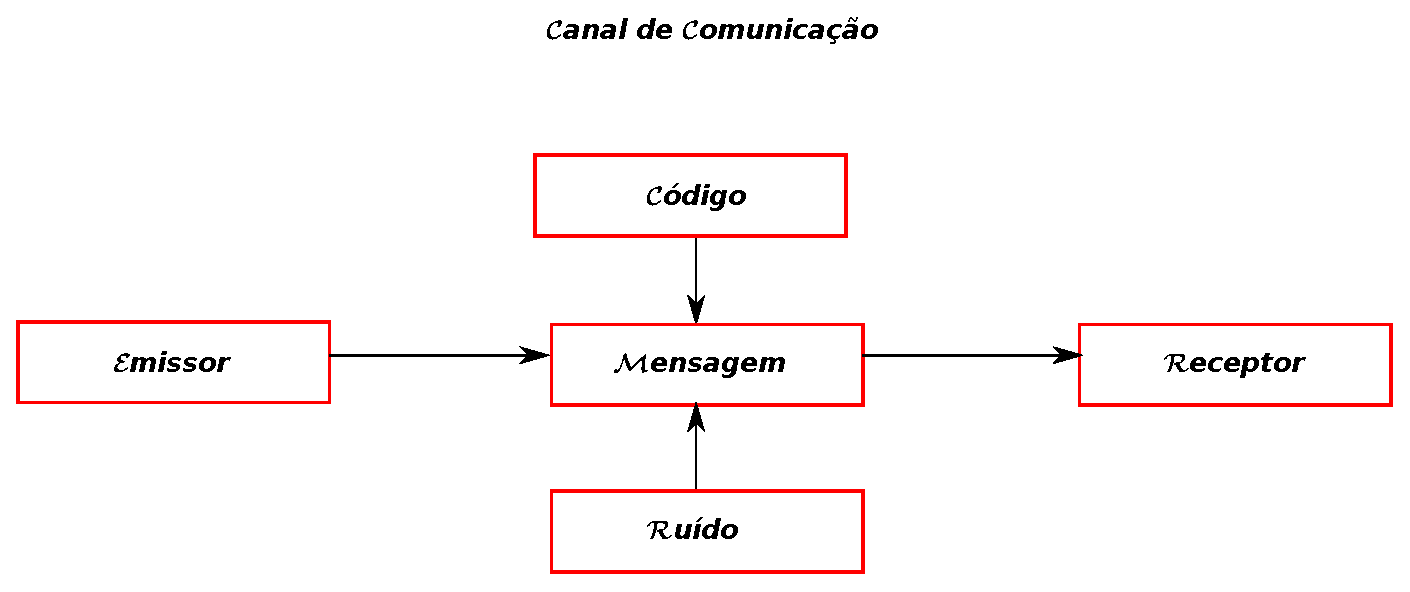
\includegraphics[width=0.50\linewidth]{../Imagens/elem_com.eps}
    \caption{Elementos do Processo de Comunicação.}\label{fig:elem_com}
   \end{figure}
\end{bigitem}
\end{frame}

\begin{frame}{Sistemas de Comunicações Atuais}
 \begin{bigitem}
  \item Como exemplo de sistemas de comunicações sem fio atuais, temos:
  \begin{bigitem}
    \item WLAN, Bluetooth, WiMAX
 \end{bigitem}
 \item Como exemplo de sistemas de comunicações móveis sem fio atuais, temos:
  \begin{bigitem}
   \item 2G, 3G, 4G.
 \end{bigitem}
 \end{bigitem}  
\end{frame}

\begin{frame}{Motivação}
 \begin{bigitem}
  \item O canal de comunicações móveis sem fio é cheio de desafios, desde a propagação até os serviços oferecidos.
  \item Para isso, é necessário um avanço nas técnicas utilizadas e nos dispositivos eletrônicos:
  \begin{bigitem}
    \item OFDM (Orthogonal Frequency-Division Multiplexing), MIMO (Multiple-Input and Multiple-Output).
    \item Microeletrônica.
  \end{bigitem}
  \item A potência de transmissão é um fator limitante em qualquer sistema de comunicações. 
 \end{bigitem}
\end{frame}

\begin{frame}{Motivação}
 \begin{bigitem}
  \item Para a nova geração, 4G, espera-se a utilização de técnicas de cooperação em conjunto com OFDM.
  \item É possível combinar técnicas de multiplexação e cooperação para um aumento da taxa de transmissão e um controle eficiente da potência de transmissão.
  \item Originam-se problemas atuais e relevantes do ponto de vista prático.
 \end{bigitem}
\end{frame}

\begin{frame}{Objetivos}
 \begin{bigitem}
  \item União de duas técnicas, multiplexação e cooperação:
  \begin{bigitem}
    \item utilização eficiente da potência de transmissão
    \item aumento da taxa.  
  \end{bigitem}
  \item É formulado um problema de otimização
  \begin{bigitem}
    \item  Objetivo:
    \begin{bigitem}
      \item  maximização da taxa
    \end{bigitem}
    \item Restrições:
    \begin{bigitem}
      \item potência em cada enlace (chamado na literatura de salto);
      \item emparelhamento dos canais (chamados de subportadoras).
    \end{bigitem}
  \end{bigitem}  
 \end{bigitem}
\end{frame}

